In this section we introduce a small example which addresses the requirements of designing a multiplayer game. We then present an architecture that aims to fulfil these requirements.

\subsection{The master/slave network architecture}

We choose to implement the networking layer in Casanova 2 by using a peer-to-peer architecture for the following reasons:

\begin{itemize}
	\item Server-client architectures are more reliable but suitable only for specific genres of games (mostly Shooter games), while other genres, such as Real-time strategy games or Online Role Playing Games use p2p architecture.
	\item We do not have to write a separate logic for an authoritative game server which has to validate the actions of clients.
\end{itemize}

Casanova will provide a generic tracking server, which is run separately from the main program. The tracking server is a thin service that connects players participating in a single game, and helps with forwarding the network traffic through NATs.

Each client maintains a local copy of the \texttt{world} entity and has direct control over a single portion of it. Instances belonging to such portion are seen as \textit{master} by this player, who is always allowed to directly change the state of the master instances without having to validate this state change by synchronizing with other players through the network.

Each client also maintains a portion of the world which is not directly under his control. Instances belonging to such portion are seen as \textit{slave} by this player, who is only allowed to \textit{predict} the local state of the instances and, whenever he receives an update from their masters, must correct this prediction according to the data contained in the received messages. The slave part of the world is thus maintained passively by the client: the only active part is predicting the evolution of the entity state and correcting it whenever he receives an update by its master.

For this purpose we extend the syntax of Casanova rules by allowing them to be marked with the modifiers \texttt{master} and \texttt{slave}. These rules are executed respectively on master and slave entities. Note that it is still possible not to mark a rule with these modifiers, which means that the rule is always executed independently of the fact that the entity is either master or slave on that particular client. We also allow to mark a rule as \texttt{connecting} and \texttt{connected}. These rules are triggered only once respectively when a new client connects and when the clients detect a new connection.

Casanova also provides primitives to send (reliably or unreliably) and receive data.

A schematic representation of this architecture can be seen in Figure \ref{fig:masterslave}.

\begin{figure}[h!]
	\centering
	\caption{Representation of the game world in a networking scenario}
	\label{fig:network_world}
	\begin{subfigure}[t]{0.3\linewidth}
		\centering
		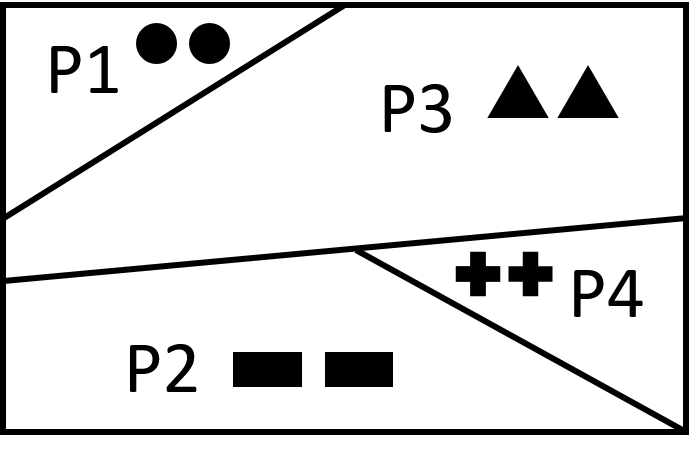
\includegraphics[width=1\linewidth]{Figures/networking2}
		\caption{Unknown correct game state when P3 joins the game.\\}
		\label{subfig:networking_ideal}
	\end{subfigure}
	\begin{subfigure}[t]{0.3\linewidth}
		\centering
		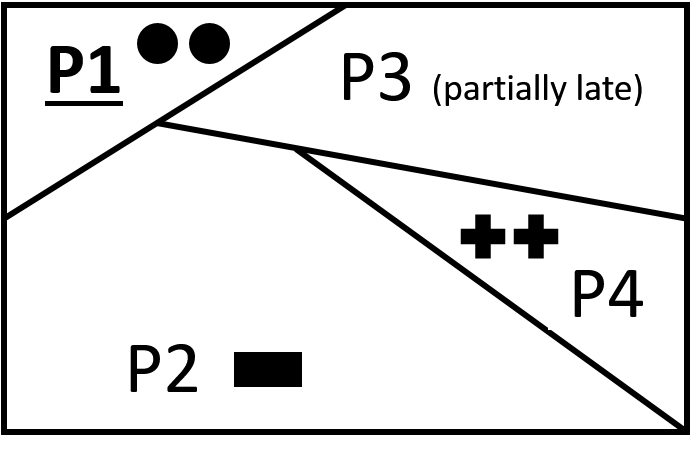
\includegraphics[width=1\linewidth]{Figures/networking1}
		\caption{Networking game state seen from the point of view of P1. P2 is partially synchronized, P4 is fully synchronized, and P3 is a new client which is late and is still sending its data}
		\label{subfig:networking_relative}
	\end{subfigure}
	

\end{figure}

\begin{figure}
	\centering
	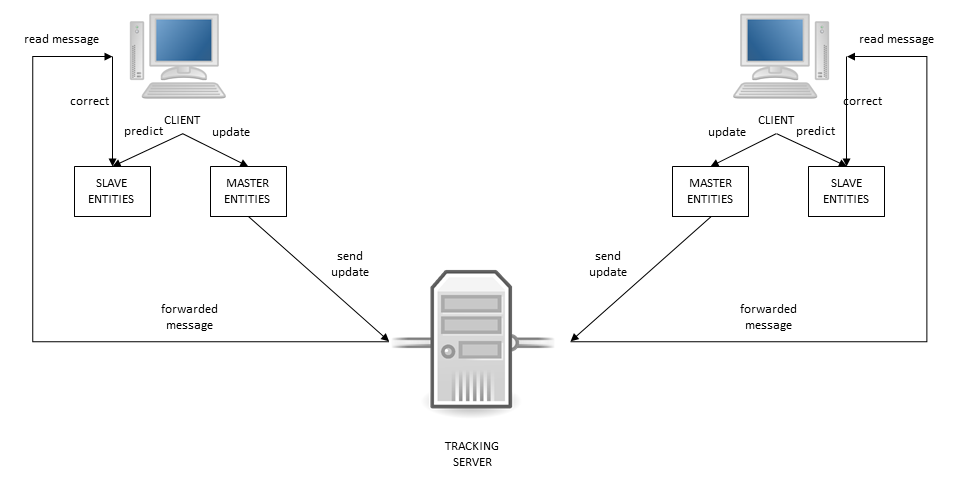
\includegraphics[scale = 0.3]{Figures/masterslave}
	\caption{master/slave architecture}
	\label{fig:masterslave}
\end{figure}

\subsection{Case study}
Let us consider a simple shooter game where each player controls a space ship. Players can move forward, backward, and rotate the ship to change direction. Moreover, they can use the ship lasers to shoot other players. If a laser hits an enemy ship we increase the player's score. Designing such a game requires to address the following issues, depicted by the schematic representation in Figure \ref{fig:network_world}:

\begin{enumerate}
	\item Each player must maintain a local version of the game state (world). In order to avoid to flood the network with messages, all the copies are not fully synchronized at each frame, thus they are slightly different and each client knows the latest version of only part of the copy.
	\item A player \texttt{connecting} to an existing game must be able to receive the latest update of the game state and send the new ship he will control to existing players in the game.
	\item A player already \texttt{connected} to the game must detect a new connection and send his master portion of the game state.
	\item Each player must be able to control only one ship at a time. This means that the part of the game logic which processes the input and modify the spatial data of the ship (position and rotation) should only be executed on the ship controlled by the player and not on the local copies of other players' ships. This means that each player sees as \texttt{master} only one ship instance.
	\item Each player must send the updated state of the ship he controls to the other players after executing the local update. To achieve better performance over the network, the data is not sent at every update, but with a lower frequency.
	\item Each player must receive the updated state of \texttt{slave} ships controlled by other players. In this phase we must take into account that, as explained above, not every update is sent so the player should ``predict'' what will happen during the game frames in which he does not receive an update.
\end{enumerate}

\subsection{Implementation}
Each of the scenarios described above requires specific language extensions. This extensions identify connection, ownership (master/slave), and various send and receive primitives. In this section we introduce each primitive by using a multiplayer game example \footnote{The game source code and executable can be found at \url{https://github.com/vs-team/casanova-mk2/wiki/Networking-extension}}. We now give an implementation of the shooter game presented above and using the extended version of Casanova 2 with network primitives. 

The \texttt{world} contains a list of ships controlled by each player.
\begin{lstlisting}
world Shooter = {
  Ships  : [Ship]
  ...
}
\end{lstlisting}

Each \texttt{Ship} contains a position, a rotation, a collection of shot projectiles, and the score.
\begin{lstlisting}
entity Ship = {
  Position   : Vector2
  Rotation   : float32
  Projectiles : [Projectile]
  Score		  : int
  ...
}

\end{lstlisting}

Each \texttt{Projectile} contains its position and velocity.

\begin{lstlisting}
entity Projectile = {
  Position : Vector2
  Velocity : Vector2
  ...
}
\end{lstlisting}

\subsubsection{Connection}
When a player connects we must consider two different situations: (\textit{i}) a player is already in the game and must send the current game state to the connecting players, and (\textit{ii}) the player who is connecting needs to send the ship he will instantiate and control (its initial state). Both the players in the game and the connecting one must receive the game states that are sent. For this purpose we introduce two additional modifiers, \texttt{connecting} and \texttt{connected}, that can be added to rule declarations to mark their role in the multiplayer logic.

\paragraph{Connecting:} A rule marked with \texttt{connecting} is executed once when a player joins the game. In our example the player should send his initial state (the created ship) to the other players. We use the primitive \texttt{send\_reliable} because we must be sure that eventually all players will be notified of the ship creation.
	\begin{lstlisting}
world Shooter = {
  ...
  rule connecting Ships =
    yield send_reliable Ships
}
	\end{lstlisting}
	
\paragraph{Connected}: A rule marked with \texttt{connected} is run whenever a new player joins the game. When this occurs, each player sends its ship. The system will take care to send only the ship controlled locally by the player itself for each player. The rule will use the \texttt{send\_reliable} primitive for the same reason explained in the previous point.

\begin{lstlisting}
world Shooter = {
  ...
  rule connected Ships =
    yield send_reliable Ships
}
\end{lstlisting}


\subsubsection{Master updates}
As explained above, each client manages a series of local game objects (called \textit{master objects}) that are under its direct control. The other clients read passively any update done on those instances and update their remote copy  (\textit{slave objects}) accordingly. We mark rules affecting the behaviour of master objects as \texttt{master}. In our example the following situations are run as master: (\textit{i}) synchronizing the ships among players, (\textit{ii}) updating the ship and projectiles spatial data, and (\textit{iii}) creating and destroying projectiles.

\begin{enumerate}[leftmargin=*,labelsep=3mm,label=\roman*]
	\item Each player is tasked to maintain the list of Ships in the world. This requires to receive the updated list from other players and to store the new value in a master rule. Indeed the world is a special case of an entity which is shared among players, and not directly owned by somebody. Each ship contained in that list and received from other players will be treated appropriately as slaves, while the only one owned by the current player will be under his direct control. In this rule we use \texttt{let!}, which is an operator which waits until the argument expression returns a result and then binds it to the variable. The rule uses \texttt{receive\_many} which receives and collects the list of sent ships by the other players.
	
	\begin{lstlisting}
world Shooter = {
  ...
  rule master Ships =
    let! ships = receive_many()
    yield Ships @ ships
}
	\end{lstlisting}
	
	\item The master version of the ship update reads the input of the player and moves (or rotates) the ship if the appropriate key is pressed. Note that this part must be executed only on a master object, because we want to allow each player to control only the ship it owns and instantiates at the beginning of the game. Below we show just the rule to move forward, the other movement and rotation rules are analogous. We use an \textit{unreliable send} because it is acceptable to lose an update of the position during a certain frame: shortly after there will be a new update.
	
	\begin{lstlisting}
entity Ship = {
  ...
  rule master Position =
    wait world.Input.IsKeyDown(Keys.W)
    let vp = new Vector2(Math.Cos(Rotation), 
                         Math.Sin(Rotation)) * 300.0f
    let p = Position + vp * dt
    yield send p
}
	\end{lstlisting}
	
	We do the same for projectiles, except the projectile position is continuously updated and synchronized over the network without having to wait that a key is pressed.
	
	\item Creating a new projectile happens when the player shoots. A ship keeps track of the projectiles it has shot so far, and adds a new one to the list of the existing projectiles. The updated list is sent to all players with the new instance of the projectile. As explained in Section \ref{sec:net_architecture}, we only send the new projectiles and not the whole list.
	
\begin{lstlisting}
entity Ship = {
  ...
  rule master Projectiles =
    wait world.Input.IsKeyDown(Keys.Space)
    let vp = new Vector2(Math.Cos(Rotation), 
                         Math.Sin(Rotation)) * 500.0f
    let projs = new Projectile(Position, vp) :: Projectiles
    yield send_reliable projs
    wait not world.Input.IsKeyDown(Keys.Space)
}
\end{lstlisting}

	Filtering the colliding projectiles and updating the score is run as a master rule. The rule computes the set difference between the ship projectiles and the colliding projectiles and updates the list of projectiles, sending them through the network as well. Even in this case, the network layer sends only the information about the projectiles to remove. Note that the score is managed by each player locally, as it does not require to be synchronized (we do not print the other players' scores. Doing so would indeed require to also send the score).
	
\begin{lstlisting}
entity Ship = {
  ...
  rule master Projectiles, Score =
    let collidingProjs =
      [for p in Projectiles do
       let ships =
         [for s in Ships do
          where s <> this and 
                Vector2.Distance(p.Position,s.Position) < 100.0f
          select s]
       where ships.Count > 0
       select p]
    let newProjectiles = Projectiles - collidingProjs
    yield send_reliable newProjectiles, 
          Score + collidingProjs.Count 
}
\end{lstlisting}
\end{enumerate}

\subsubsection{Managing remote instances}
The game objects that were not instantiated by a client, but received from another client, are \textit{slave objects} and must be synchronized differently than master objects. For this purpose, a rule can be marked as \texttt{slave}. In our example we use slave rules in the following situations: (\textit{i}) synchronizing other players' ships and projectiles spatial data, and (\textit{ii}) projectiles instantiated by other players.

\begin{enumerate}[leftmargin=*,labelsep=3mm,label=\roman*]
	\item Every remote projectile and ship is synchronized locally by a rule which tries to \texttt{receive} a message containing updated special data. Below we provide the code to update the position of the ship, the synchronization of other spacial data is analogous.
	
\begin{lstlisting}
  entity Ship = {
  ...
  rule slave Position = yield receive()
}
\end{lstlisting}
	
	\item When a projectile is instantiated remotely, we have to receive it and add it to the list of projectiles. We use \texttt{receive\_many} because the new projectiles are added to a list. This case also supports the situation where a ship could shoot multiple projectiles at the same time.
	
\begin{lstlisting}
entity Ship = {
  ...
  rule slave Projectiles =
    let! projs = receive_many()
    yield projs @ Projectiles
}
\end{lstlisting} 
\end{enumerate}